% Provenance (never printed): see sources/outline_sources.md (Year 1: litho-, bio- and
% chronostratigraphy; boundary stratotypes; mass extinctions as global markers; the
% international chart). Exercise and problem values in the Book 3 scratch calculator
% calc/ch24.py; the chart from figdata/bachelor-1/ics_chart.py (shared ics rows).
% The principles of relative dating, eras and periods are Book 1's (g7 geological-time) and
% are re-founded here. Mass extinctions belong to the biology series (recalled in prose);
% their Earth causes are the Year 2 volume's (phanerozoic-earth). Correlation of logs and
% unconformities are ch. 5's; facies ch. 21's; compaction ch. 23's. Radiometric dating is
% ch. 25's. Sequence stratigraphy, facies models and Walther's law are the Year 3 volume's;
% magnetostratigraphy too: prose pointers only. "Transgression" is explained in prose.
\chapter{De stratigrafische schaal}\label{ch:b1:stratigraphic-scale}

Op het strand van Itzurun, bij Zumaia aan de Baskische kust, bestaan de kliffen uit dunne lagen kalksteen en mergel, gekanteld en honderden meters lang herhaald. Op één contact, waar een bleke kalksteenlaag eindigt en rode mergels beginnen, is een bronzen schijfje met vier letters in het gesteente gezet (figuur hieronder). Het is een gouden spijker. Zij legt voor de hele planeet het moment vast waarop één indeling van de geologische tijd --- de \omterm{def:b1:stratigraphic-scale:chronostratigraphy}{etage} Selandien --- begint. Een gesteente in Patagonië of in Siberië is Selandiaans als het werd afgezet na het moment dat op dat contact is vastgelegd en vóór het moment dat op de volgende spijker hoger op de schaal wordt vastgelegd. Dit hoofdstuk legt uit waarom geologen zo'n merkteken nodig hadden: drie verschillende manieren om een stapel gesteenten in te delen, de principes die ze ordenen, de lijnen die ver uiteenliggende secties verbinden, en de internationale schaal die het resultaat samenbrengt.

\begin{omfigure}
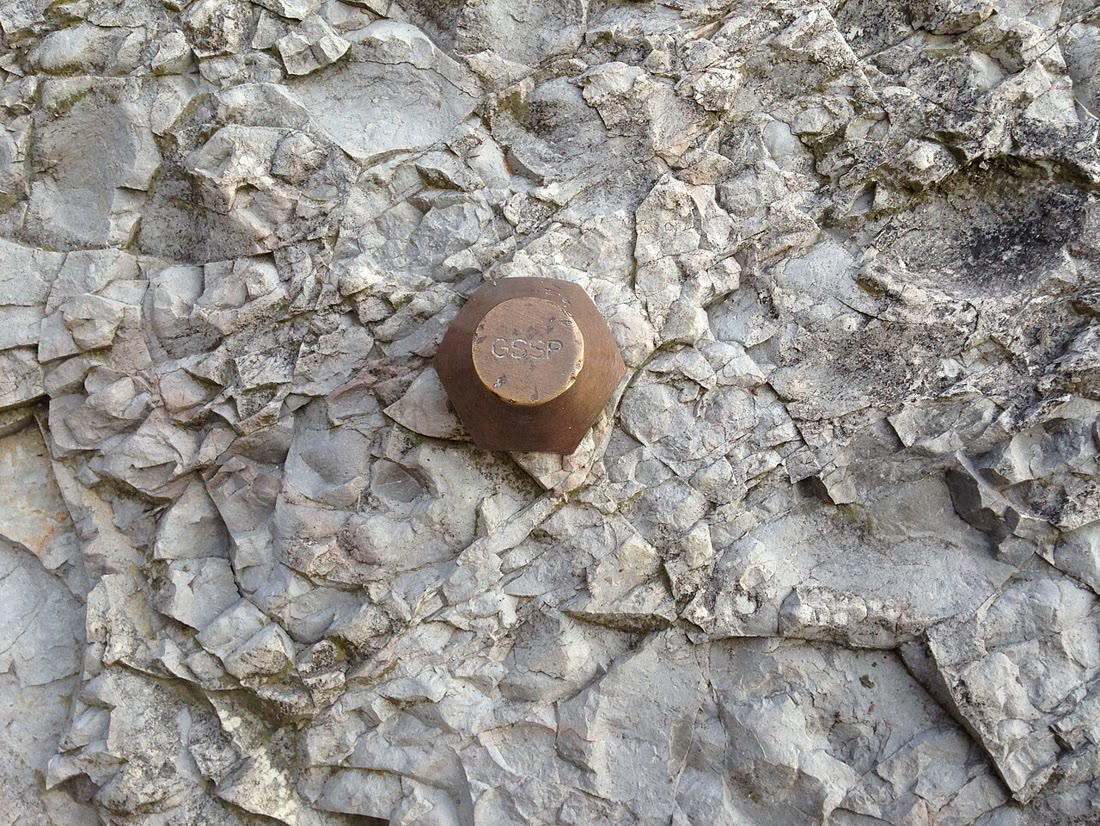
\includegraphics[width=0.62\linewidth]{images/book3/b1-golden-spike-zumaia.jpg}

{\small De gouden spijker van de \omterm{def:b1:stratigraphic-scale:chronostratigraphy}{etage} Selandien in de sectie van Zumaia: een bronzen merkteken met de letters GSSP, geplaatst op de top van de bovenste kalksteenlaag van één \omterm{def:b1:stratigraphic-scale:lithostratigraphy}{formatie}, aan de basis van de rode mergels van de volgende. (Josugoni, CC~BY-SA~4.0, via Wikimedia Commons.)}
\label{fig:b1:stratigraphic-scale:zumaia}
\end{omfigure}
% ledger: commons:zumaia-gssp, gssp:selandian

\begin{recall}
In een stapel lagen die niet is omgekeerd, is elke laag jonger dan die eronder; een structuur die gesteenten doorsnijdt, is jonger dan zij; fossielen veranderen van oudere lagen naar jongere in overal dezelfde volgorde; de geschiedenis van de aarde is verdeeld in tijdperken en geologische perioden, elk met een leeftijd in jaren voor zijn begin, verzameld in een internationale schaal (Boek~1, klas~7). Een boorlog registreert de eenheden die tegen de diepte zijn aangetroffen, en correlatie koppelt dezelfde eenheden van log tot log (\cref{def:b1:cross-sections:log}); een \omterm{def:b1:cross-sections:unconformity}{discordantie} is een oppervlak van erosie of niet-afzetting (\cref{def:b1:cross-sections:unconformity}). Een \omterm{def:b1:clastic-sediments:facies}{sedimentaire facies} is een gesteentelichaam waarvan de kenmerken het milieu van afzetting registreren (\cref{def:b1:clastic-sediments:facies}). De biologievolumes beschrijven hoe soorten verschijnen en uitsterven, en de weinige massa-extincties waarbij binnen korte tijd een groot deel van alle soorten verdween.
\end{recall}

\section{Drie manieren om de gesteenten in te delen}\label{sec:b1:stratigraphic-scale:three}

Een geoloog die een klif logt kan dezelfde stapel lagen op drie manieren indelen: naar waaruit de gesteenten bestaan, naar de fossielen die zij bevatten, en naar de tijd waarin zij werden afgezet. De drie indelingen beantwoorden verschillende vragen, en hun grenzen hoeven niet samen te vallen. De regels voor het benoemen en definiëren van elk soort eenheid worden vastgelegd bij internationale overeenkomst.
% ledger: isg:lithostratigraphy

\begin{definition}[Formatie, lid, groep]\label{def:b1:stratigraphic-scale:lithostratigraphy}
Een \emph{lithostratigrafische eenheid}\index{lithostratigrafische eenheid} is een gesteentelichaam dat wordt gedefinieerd en herkend aan zijn lithologie en zijn positie ten opzichte van andere lichamen, wat zijn leeftijd ook is. De primaire eenheid is de \emph{formatie}\index{formatie (lithostratigrafisch)}: een gesteentelichaam dat voldoende verschilt van zijn buren om op regionale schaal in kaart te worden gebracht, en waarin de hele kolom moet worden verdeeld. Een \emph{lid}\index{lid (lithostratigrafisch)} is een benoemde onderverdeling van een formatie, onderscheiden door haar lithologie; een \emph{groep}\index{groep (lithostratigrafisch)} is een opeenvolging van twee of meer formaties met belangrijke lithologische kenmerken gemeen. Een formele naam verbindt een lokale geografische naam met de rang of met het overheersende gesteente: de Kell Sandstone, de Mardon Shale Formation.
\end{definition}
% ledger: isg:lithostratigraphy

Een \omterm{def:b1:stratigraphic-scale:lithostratigraphy}{formatie} kan minder dan een meter dik zijn of enkele duizenden meters. Zij wordt van haar typesectie af alleen zo ver uitgebreid als haar lithologie kan worden herkend, zodat haar grenzen het gesteente volgen, niet de tijd.
% ledger: isg:lithostratigraphy

\begin{definition}[Biozone, indexfossiel, eerste-voorkomenshorizont]\label{def:b1:stratigraphic-scale:biozone}
Een \emph{biozone}\index{biozone} is een lichaam van lagen dat wordt gedefinieerd of gekenmerkt door de fossielen die het bevat. Een \emph{bereikzone}\index{bereikzone} omvat de bekende voorkomens van één taxon; een \emph{intervalzone}\index{intervalzone} is het lichaam van lagen tussen twee gespecificeerde fossielhorizonten, bijvoorbeeld de laagste voorkomens van twee taxa. De \emph{eerste-voorkomenshorizont}\index{eerste-voorkomenshorizont} (FAD) van een taxon is de horizont van zijn laagste voorkomen, de \emph{laatste-voorkomenshorizont}\index{laatste-voorkomenshorizont} die van zijn hoogste. Een \emph{indexfossiel}\index{indexfossiel} is een taxon dat wordt gebruikt om een biozone te herkennen: de beste zijn wijdverspreid, talrijk, gemakkelijk te herkennen en kortlevend.
\end{definition}
% ledger: isg:biostratigraphy, og:stratigraphy-principles

Een fossielhorizont heeft geen dikte; een \omterm{def:b1:stratigraphic-scale:biozone}{biozone} kan enkele meters of enkele honderden meters dik zijn, afhankelijk van hoe snel het sediment zich ophoopte terwijl de taxa leefden. Omdat soorten evolueren en nooit weer verschijnen zodra zij zijn uitgestorven, is de assemblage van elke leeftijd uniek. Enkele van de beste \omterm{def:b1:stratigraphic-scale:biozone}{indexfossielen} zijn microfossielen, zoals foraminiferen en conodonten: wijdverspreid, talrijk, en klein genoeg om uit de boorspaanders van een put te worden teruggevonden.
% ledger: isg:biostratigraphy, og:stratigraphy-principles

\begin{definition}[Chronostratigrafische en geochronologische eenheden]\label{def:b1:stratigraphic-scale:chronostratigraphy}
Een \emph{chronostratigrafische eenheid}\index{chronostratigrafische eenheid} is het lichaam van alle gesteenten die tijdens een gegeven interval van de geologische tijd zijn gevormd, en alleen tijdens dat interval; haar grenzen zijn oppervlakken van gelijke leeftijd. Het tijdinterval zelf is een \emph{geochronologische eenheid}\index{geochronologische eenheid}. De rangen, van de kleinste af, zijn de \emph{etage}\index{etage (chronostratigrafisch)} (zijn tijd: een leeftijd), de \emph{serie}\index{serie (chronostratigrafisch)} (een tijdvak), het \emph{systeem}\index{systeem (chronostratigrafisch)} (een periode), het erathema (een tijdperk) en het eonothema (een eon); elke eenheid bestaat uit verschillende opeenvolgende eenheden van de rang eronder.
\end{definition}
% ledger: isg:chronostratigraphy

De twee woorden beschrijven dezelfde indeling gezien als gesteente of als tijd (\cref{tab:b1:stratigraphic-scale:ranks}): gesteenten van het Jura-systeem werden afgezet tijdens de Jura-periode, en de Lager-Jura-serie tijdens het Vroeg-Jura-tijdvak. De \omterm{def:b1:stratigraphic-scale:chronostratigraphy}{etage} is de kleinste eenheid die overal ter wereld wordt herkend.
% ledger: isg:chronostratigraphy, chart:danian

\begin{table}[htbp]
\centering
\begin{tabular}{lll}
\hline
\shortstack[l]{chrono\-stratigrafische\\eenheid (gesteente)} & \shortstack[l]{geo\-chronologische\\eenheid (tijd)} & voorbeeld \\
\hline
eonothema & eon    & Fanerozoïcum \\
erathema  & tijdperk & Cenozoïcum \\
systeem   & periode & Paleogeen \\
\omterm{def:b1:stratigraphic-scale:chronostratigraphy}{serie}     & tijdvak  & Paleoceen \\
\omterm{def:b1:stratigraphic-scale:chronostratigraphy}{etage}     & leeftijd & Danien (\qtyrange{66.00}{61.66}{\Ma}) \\
\hline
\end{tabular}
\caption{De rangen van de chronostratigrafische en geochronologische eenheden, met de eenheden die het Danien bevatten, de eerste \omterm{def:b1:stratigraphic-scale:chronostratigraphy}{etage} van het Cenozoïcum.}
\label{tab:b1:stratigraphic-scale:ranks}
\end{table}
% ledger: isg:chronostratigraphy, chart:danian

\section{De principes en de correlatie}\label{sec:b1:stratigraphic-scale:principles}

Voordat een gesteente in jaren kon worden gedateerd, werd de volgorde van gebeurtenissen uit de gesteenten zelf afgelezen. De basisprincipes van de stratigrafie werden in 1669 door Nicolas Steno uiteengezet; tussen 1785 en 1800 voegden Hutton en William Smith het gebruik van de lagen als tijdintervallen toe, en van hun fossielen om ze te herkennen.
% ledger: og:stratigraphy-principles, usgs:hutton-smith

\begin{definition}[Principes van de stratigrafie]\label{def:b1:stratigraphic-scale:principles}
\begin{enumerate}
  \item Het \emph{superpositieprincipe}\index{superpositieprincipe}: in een reeks sedimentaire lagen die niet is omgekeerd, is elke laag jonger dan die waarop zij rust.
  \item Het \emph{principe van oorspronkelijke horizontaliteit}\index{oorspronkelijke horizontaliteit, principe van}: sedimenten en lavastromen worden horizontaal of bijna horizontaal afgezet --- aan de randen van een bekken licht hellend.
  \item Het \emph{principe van laterale continuïteit}\index{laterale continuïteit, principe van}: binnen een bekken loopt een laag ononderbroken in elke richting tot zij aan de rand van het bekken of tegen een obstakel uitdunt; een laag die door een dal is doorsneden, zet zich aan de andere kant voort.
  \item Het \emph{principe van de doorsnijdingsrelaties}\index{doorsnijdingsrelaties, principe van}: een lichaam of structuur dat gesteenten doorsnijdt --- een dijk, een breuk, een erosieoppervlak --- is jonger dan de gesteenten die het doorsnijdt.
  \item Het \emph{principe van faunale opvolging}\index{faunale opvolging, principe van}: fossiele taxa volgen elkaar in dezelfde volgorde op in elke regio, zodat gesteenten met dezelfde assemblage van dezelfde leeftijd zijn.
\end{enumerate}
\end{definition}
% ledger: og:stratigraphy-principles, eli:relative-dating, usgs:fossil-succession, isg:chronostratigraphy

De principes zijn niet even sterk. Superpositie geeft een volgorde die elke andere methode moet respecteren. Oorspronkelijke horizontaliteit maakt dat een gekantelde laag een registratie van latere vervorming is. Laterale continuïteit laat een geoloog dezelfde laag aan beide zijden van een dal tekenen, en binnen een beperkte afstand is een op de grond gevolgd gelaagdheidsvlak de beste lijn van gelijke leeftijd die er is. Faunale opvolging is het principe dat oceanen oversteekt; zij is het onderwerp van de volgende alinea's.
% ledger: isg:chronostratigraphy, og:stratigraphy-principles

\subsection*{Correlatie door biozones}

\omterm{def:b1:cross-sections:log}{Correlatie} door fossielen vergelijkt de volgorde van eerste en laatste voorkomens in twee secties (figuur hieronder). De twee zijn niet even betrouwbaar. Het hoogste fossiel van een taxon dat in een sectie wordt gevonden, hangt af van hoeveel er zijn bewaard: waar zij zeldzaam zijn, kan het laatst gevonden exemplaar ver onder het niveau liggen waarop het taxon werkelijk verdween, en een fossiel dat werd geërodeerd en opnieuw afgezet, kan erboven opduiken. Een eerste voorkomen kan ook verschuiven, maar een wijdverspreid taxon dat zich snel verspreidde, wordt in een bekken op ongeveer hetzelfde niveau bereikt.
% ledger: isg:biostratigraphy

\begin{omfigure}
\begin{tikzpicture}[font=\footnotesize, y=0.13cm]
  % section 1: 40 m, sandstone 0-14, shale 14-40
  \fill[lith sandstone] (0,0) rectangle (0.8,14);
  \fill[lith shale] (0,14) rectangle (0.8,40);
  \draw[black!70] (0,0) rectangle (0.8,40);
  \node[anchor=south, font=\small] at (1.4,41.5) {sectie 1};
  \foreach \x/\a/\b/\t in {1.1/0/27/a, 1.4/10/34/b, 1.7/20/40/c, 2.0/30/40/d} {
    \draw[line width=2.2pt, omThm] (\x,\a) -- (\x,\b);
    \node[anchor=base, font=\scriptsize] at (\x,-4.5) {\t};
  }
  \foreach \y/\z in {5/a, 15/b, 25/c, 35/d}
    \node[anchor=east, font=\scriptsize] at (-0.1,\y) {zone \z};
  \foreach \y in {10,20,30} \draw[black!50] (-1.3,\y) -- (0,\y);
  % scale bar
  \draw[thick] (-1.5,0) -- (-1.5,10) node[midway, anchor=east, font=\scriptsize] {\qty{10}{m}};
  % section 2: 24 m, sandstone 0-3, shale 3-24
  \begin{scope}[xshift=7cm]
    \fill[lith sandstone] (0,0) rectangle (0.8,3);
    \fill[lith shale] (0,3) rectangle (0.8,24);
    \draw[black!70] (0,0) rectangle (0.8,24);
    \node[anchor=south, font=\small] at (1.4,25.5) {sectie 2};
    \foreach \x/\a/\b/\t in {1.1/0/13/a, 1.4/6/20/b, 1.7/12/24/c, 2.0/18/24/d} {
      \draw[line width=2.2pt, omThm] (\x,\a) -- (\x,\b);
      \node[anchor=base, font=\scriptsize] at (\x,-4.5) {\t};
    }
    \foreach \y/\z in {3/a, 9/b, 15/c, 21/d}
      \node[anchor=west, font=\scriptsize] at (2.3,\y) {zone \z};
    \foreach \y in {6,12,18} \draw[black!50] (0.8,\y) -- (2.3,\y);
  \end{scope}
  % correlation of the first appearances
  \foreach \u/\v/\t in {10/6/b, 20/12/c, 30/18/d}
    \draw[densely dashed, omThm!70!black] (2.15,\u) -- (6.85,\v)
      node[pos=0.5, fill=white, inner sep=1pt, font=\scriptsize] {FAD \t};
\end{tikzpicture}

{\small Een bereikschema en een correlatie door \omterm{def:b1:stratigraphic-scale:biozone}{biozones} (verzonnen taxa \emph{a} tot \emph{d}). De dikke balken zijn de bereiken van de taxa in elke sectie. Drie \omterm{def:b1:stratigraphic-scale:biozone}{intervalzones} worden begrensd door de eerste voorkomens van \emph{b}, \emph{c} en \emph{d}, die van sectie tot sectie worden verbonden (gestreept). Het laatste voorkomen van \emph{a} valt in het bovenste deel van zone~\emph{c} in sectie~1 en nabij de basis in sectie~2: het is een slechtere gids. De zones zijn dunner in sectie~2, waar het sediment langzamer ophoopte.}
\label{fig:b1:stratigraphic-scale:range-chart}
\end{omfigure}

\begin{method}[Correlatie van secties via biozones]\label{met:b1:stratigraphic-scale:biozones}
\begin{enumerate}
  \item Zet voor elke sectie het bereik van elk taxon uit tegen de hoogte: van zijn laagste tot zijn hoogste voorkomen.
  \item Kies de fossielhorizonten die de zones bepalen --- bij voorkeur eerste voorkomens van wijdverspreide taxa die onafhankelijk zijn van de facies.
  \item Teken de zonegrenzen in elke sectie op deze horizonten.
  \item Verbind dezelfde horizonten van sectie tot sectie; controleer dat de lijnen elkaar niet kruisen, zoals superpositie vereist.
  \item Lees tussen twee lijnen de dikte van elke zone in elke sectie af; waar een zone ontbreekt, zoek naar een \omterm{def:b1:cross-sections:unconformity}{discordantie} of een verandering van facies voordat men besluit dat het taxon afwezig is.
\end{enumerate}
\end{method}

Een \omterm{def:b1:stratigraphic-scale:biozone}{biozone} is slechts zo goed als de onafhankelijkheid van haar fossielen van het milieu. Een tweekleppige die alleen op zandige kusten leefde, wordt alleen in zandsteen gevonden; hem van sectie tot sectie volgen, volgt het zandsteen, niet de tijd. Biostratigrafische correlatie is daarom niet noodzakelijk tijdcorrelatie: zij kan een facies volgen waarvan de leeftijd van plaats tot plaats verandert.
% ledger: isg:biostratigraphy

\subsection*{Grenzen die door de tijd snijden}

Verschillende sedimenten worden op verschillende plaatsen tegelijk afgezet: zand op de kust, slib uit zee, kalk verder weg op een plat dat van zand verstoken is. Een lijn van gelijke leeftijd loopt daarom van de ene lithologie naar de andere. Omgekeerd hoeft een lithologische grens die over een bekken wordt getrokken, helemaal geen lijn van gelijke leeftijd te zijn.
% ledger: og:stratigraphy-principles, isg:chronostratigraphy

\begin{definition}[Diachrone grens]\label{def:b1:stratigraphic-scale:diachronous}
Een grens is \emph{diachroon}\index{diachrone grens} wanneer haar leeftijd langs haar van plaats tot plaats verandert. De grenzen van \omterm{def:b1:stratigraphic-scale:lithostratigraphy}{formaties} en van facies zijn gewoonlijk diachroon; de grenzen van chronostratigrafische eenheden zijn dat per definitie niet.
\end{definition}
% ledger: isg:lithostratigraphy, isg:chronostratigraphy, isg:biostratigraphy

Het klassieke geval is een transgressie: het \omterm{def:b1:diagenesis-basins:eustasy}{relatief zeeniveau} stijgt sneller dan het sediment de gemaakte ruimte kan vullen, en de kustlijn verschuift landinwaarts. Het strandzand wordt op elk moment aan de kustlijn afgezet, dus verspreidt een zandsteenlaag zich landinwaarts met haar mee; het slib uit zee volgt erbovenop. De top van het zandsteen is dan het spoor van de bewegende kustlijn: jong landinwaarts, oud zeewaarts (figuur hieronder). De volgorde van facies die in één verticale doorsnede wordt gezien --- zandsteen onder schalie onder kalksteen --- herhaalt hun volgorde over het plat op één moment; Boek~5 maakt hiervan de basis van zijn faciesmodellen.
% ledger: og:stratigraphy-principles, isg:lithostratigraphy

\begin{omfigure}
\begin{tikzpicture}[font=\footnotesize, x=1cm, y=1cm]
  % basement surface B(x) = 1.6 (1 - x/14), rising towards the land on the left
  \fill[lith granite] (0,-0.5) -- (0,1.6) -- (14,0) -- (14,-0.5) -- cycle;
  \fill[lith sandstone] (0,1.6) -- (14,0) -- (14,0.5) -- (0,2.1) -- cycle;
  \fill[lith shale] (0,2.1) -- (14,0.5) -- (14,1.5) -- (0,3.1) -- cycle;
  \fill[lith limestone] (0,3.1) -- (14,1.5) -- (14,3.6) -- (0,3.6) -- cycle;
  \draw[unconformity] (0,1.6) -- (14,0);
  \draw[black!70] (0,2.1) -- (14,0.5) (0,3.1) -- (14,1.5);
  \draw[black!70] (0,-0.5) rectangle (14,3.6);
  % time lines: horizontal, from the basement (or the left edge) to the right edge
  \foreach \y/\t in {0.6/1, 1.1/2, 1.6/3, 2.1/4, 2.6/5, 3.1/6} {
    \pgfmathsetmacro{\xs}{max(0, 14*(1-\y/1.6))}
    \draw[omThm, thick, densely dashed] (\xs,\y) -- (14,\y) node[anchor=west, text=black] {$t_\t$};
  }
  % two sections
  \foreach \x/\n in {3/1, 11/2} {
    \draw[very thick, black] (\x,-0.5) -- (\x,3.6);
    \node[anchor=south, font=\small] at (\x,3.65) {sectie \n};
  }
  \node[fill=white, inner sep=1pt, font=\scriptsize] at (5.6,1.21) {zandsteen};
  \node[fill=white, inner sep=1pt] at (12.6,1.2) {schalie};
  \node[fill=white, inner sep=1pt] at (7.0,3.25) {kalksteen};
  \node[fill=white, inner sep=1pt] at (12.0,-0.25) {basement};
  \draw[-{Stealth}, thick] (5.6,4.35) -- (3.6,4.35) node[anchor=east] {land};
  \draw[-{Stealth}, thick] (8.4,4.35) -- (10.4,4.35) node[anchor=west] {zee};
\end{tikzpicture}

{\small Een zandsteenlaag afgezet tijdens een transgressie (schematisch, verticale schaal overdreven). De gestippelde lijnen $t_1$ tot $t_6$ verbinden punten van gelijke leeftijd, $t_1$ de oudste. Waar een lijn het basement raakt, begint zij aan de kustlijn van haar tijd; zeewaarts gaat zij van zand over in slib en, in de jongere, in kalk. De top van het zandsteen ligt in sectie~2 tussen $t_1$ en $t_2$, maar in sectie~1 tussen $t_3$ en $t_4$: de grens van de \omterm{def:b1:stratigraphic-scale:lithostratigraphy}{formatie} is \omterm{def:b1:stratigraphic-scale:diachronous}{diachroon}, jonger naar het land toe.}
\label{fig:b1:stratigraphic-scale:diachronous}
\end{omfigure}

Hoe snel verandert de leeftijd van de grens langs haar? Op een kustvlakte die langzaam landinwaarts stijgt, is het antwoord een kwestie van meetkunde.

\begin{proposition}[Snelheid van een transgressie]\label{prop:b1:stratigraphic-scale:transgression}
Een kustvlakte stijgt landinwaarts met de uniforme helling $s$, en het \omterm{def:b1:diagenesis-basins:eustasy}{relatief zeeniveau} stijgt met de constante snelheid $R$, zonder dat er sediment aan de kust wordt toegevoegd. De kustlijn beweegt zich dan landinwaarts met de snelheid
\[
  u = \frac{R}{s},
\]
en een grens die de kustlijn volgt, is op een punt op een afstand $d$ verder landinwaarts jonger, met $\Delta t = d/u = d\,s/R$.
\end{proposition}

\begin{proof}
Neem $x$ als de afstand landinwaarts vanaf een vast punt en $z$ als de hoogte; de vlakte is de lijn $z = s x$, en het zeeoppervlak op tijdstip $t$ is $z = z_0 + R t$. De kustlijn ligt waar zij elkaar ontmoeten: $s\,x(t) = z_0 + R t$, dus $x(t) = (z_0 + R t)/s$ en $\mathrm dx/\mathrm dt = R/s$. De kustlijn bereikt een punt op een afstand $d$ verder landinwaarts na de tijd $d/u = d\,s/R$.
\end{proof}

De verhouding is groot omdat kustvlakten bijna vlak zijn. Een stijging van \qty{10}{m} per miljoen jaar over een vlakte die $1$ op $2000$ helt, verplaatst de kust \qty{20}{km} landinwaarts per miljoen jaar; een zandsteentop die in een klif als één oppervlak lijkt, is dan een miljoen jaar jonger \qty{20}{km} landinwaarts. Sediment dat naar de kust wordt aangevoerd, vertraagt de transgressie of keert haar om.

\subsection*{Lijnen van gelijke leeftijd}

Wat correleert dan de tijd, als de lithologie dat niet doet en fossielen dat slechts bij benadering doen? De beste lijnen worden gemaakt door gebeurtenissen die overal tegelijk een spoor achterlaten. Een vulkanische as valt over een breed gebied in wat geologisch gezien een ogenblik is, en bezinkt op zand, slib en kalk gelijkelijk: een asbed is een lijn van gelijke leeftijd die faciesgrenzen doorkruist, en zij kan vaak in jaren worden gedateerd met de methoden van \cref{ch:b1:radiometric-methods}. Omkeringen van het magnetisch veld van de aarde, die in Boek~5 aan bod komen, worden geregistreerd in gesteenten van vele soorten en kunnen wereldwijd worden herkend zodra hun volgorde bekend is; dat geldt ook voor scherpe verschuivingen in de isotopen van koolstof, zoals die welke de basis van het Ypresien markeert (\cref{tab:b1:stratigraphic-scale:gssps}). Tussen twee gedateerde niveaus wordt de leeftijd van elke laag geschat door aan te nemen dat het sediment met een constante snelheid ophoopte.
% ledger: isg:chronostratigraphy

\begin{proposition}[Leeftijd tussen twee gedateerde niveaus]\label{prop:b1:stratigraphic-scale:interpolation}
Twee lagen op de hoogten $z_1 < z_2$ van een continue sectie hebben de leeftijden $t_1 > t_2$. Als het sediment er tussen met een constante snelheid is opgehoopt, heeft een niveau op de hoogte $z$ ertussen de leeftijd
\[
  t = t_1 - f\,(t_1 - t_2), \qquad f = \frac{z - z_1}{z_2 - z_1},
\]
en de accumulatiesnelheid is $r = (z_2 - z_1)/(t_1 - t_2)$. Als de twee leeftijden de onafhankelijke standaardonzekerheden $\sigma_1$ en $\sigma_2$ dragen, draagt de geïnterpoleerde leeftijd de onzekerheid
\[
  \sigma_t = \sqrt{(1 - f)^2 \sigma_1^2 + f^2 \sigma_2^2}.
\]
\end{proposition}

\begin{proof}
Bij een constante snelheid $r$ groeit de hoogte lineair met de tijd: $z - z_1 = r\,(t_1
- t)$, aangezien leeftijden naar boven afnemen. Bij $z_2$ geldt $z_2 - z_1 = r\,(t_1 - t_2)$, wat
$r$ geeft; het delen van de twee betrekkingen geeft $t_1 - t = f\,(t_1 - t_2)$. De leeftijd
is de lineaire combinatie $t = (1 - f)\,t_1 + f\,t_2$ van twee onafhankelijke
grootheden; de variantie van $a X + b Y$ voor onafhankelijke $X$ en $Y$ is $a^2
\operatorname{Var} X + b^2 \operatorname{Var} Y$, wat $\sigma_t$ geeft.
\end{proof}

De onzekerheid is het kleinst tussen de twee gedateerde lagen en is er nooit groter dan de grootste van $\sigma_1$ en $\sigma_2$. De echte grens is de aanname: sediment hoopt zich op in pulsen, kan stoppen bij verborgen breuken, en compacteert verschillend in zand en in slib (\cref{prop:b1:diagenesis-basins:solid}), zodat de geïnterpoleerde leeftijd niet beter is dan de regelmatigheid van de sectie.

\section{Grensstratotypen}\label{sec:b1:stratigraphic-scale:gssp}

Een \omterm{def:b1:stratigraphic-scale:chronostratigraphy}{chronostratigrafische eenheid} wordt in het gesteente gedefinieerd voordat zij wordt gedateerd. De oudere praktijk beschreef elke \omterm{def:b1:stratigraphic-scale:chronostratigraphy}{etage} aan de hand van een typesectie van de hele eenheid; maar de top van de ene typesectie en de basis van de volgende, op verschillende plaatsen gekozen, konden tussen hen een kloof van niet-toegewezen tijd laten of elkaar overlappen. De moderne praktijk definieert slechts de onderste grens van elke eenheid op één punt in één sectie; de bovenste grens is de onderste grens van de volgende eenheid. Er kan dan geen tijdinterval tussen twee eenheden vallen of tot beide behoren.
% ledger: isg:stratotype, isg:chronostratigraphy

\begin{definition}[Grensstratotype, eenheidsstratotype, GSSP]\label{def:b1:stratigraphic-scale:gssp}
Een \emph{stratotype}\index{stratotype} is de aangewezen gesteentesectie die dient als standaard van referentie voor een eenheid of een grens. Een \emph{eenheidsstratotype}\index{eenheidsstratotype} is de typesectie van een hele eenheid; een \emph{grensstratotype}\index{grensstratotype} is de sectie die het specifieke punt bevat dat een grens tussen twee eenheden definieert. Een \emph{global boundary
stratotype section and point}\index{global boundary stratotype section and point (GSSP)} (GSSP) is het grensstratotype van een eenheid van de internationale chronostratigrafische schaal: één punt in één sectie, gekozen bij internationale overeenkomst, dat de basis van een \omterm{def:b1:stratigraphic-scale:chronostratigraphy}{etage} en van elke grotere eenheid die ermee begint definieert.
\end{definition}
% ledger: isg:stratotype, isg:chronostratigraphy, gssp:protocol

Het GSSP is een punt in het gesteente, geen leeftijd. Zijn leeftijd in jaren is wat de beste datering van dat punt geeft, en zij kan worden verfijnd zonder het punt te verplaatsen. De sectie wordt zo gekozen dat het punt elders vindbaar is: de afzetting is continu over de grens (nooit bij een \omterm{def:b1:cross-sections:unconformity}{discordantie}, waar de ontbrekende tijd de grens dubbelzinnig zou maken), bij voorkeur mariene, rijk aan goed bewaarde fossielen van wijdverspreide taxa, zonder verandering van facies op het niveau, weinig vervormd of veranderd, toegankelijk en beschermd. Vooral wordt het punt gelegd op een niveau dat samenvalt met één gekozen signaal --- meestal het eerste voorkomen van een taxon --- binnen een interval dat rijk is aan andere signalen (asbedden, magnetische omkeringen, isotopenverschuivingen), waarmee het niveau van ver weg kan worden herkend. Op het punt wordt een blijvend merkteken geplaatst, de gouden spijker.
% ledger: isg:chronostratigraphy, isg:stratotype, gssp:protocol

\begin{inthefield}[Hoe een grens wordt gekozen]
Een grens wordt bestudeerd door een werkgroep van de subcommissie die verantwoordelijk is voor het systeem, die kandidaatsecties vergelijkt, ze laag voor laag logt, hun fossielen, asbedden en isotopen bemonstert, en een voorstel schrijft. Een voorstel heeft een supermeerderheid nodig --- meer dan \qty{60}{\%} --- van de stemgerechtigde leden van de subcommissie, ongeveer twintig specialisten; het gaat dan naar de stemgerechtigde leden van de Internationale Commissie voor Stratigrafie, de uitvoerende functionarissen en de voorzitters van haar zeventien subcommissies, en ten slotte naar het uitvoerend comité van de Internationale Unie van Geologische Wetenschappen, dat de grens bekrachtigt. De resultaten worden gepubliceerd, het merkteken wordt in het gesteente gezet, en er mag tien jaar lang geen wijziging van een pas vastgestelde grens worden voorgesteld.
\end{inthefield}
% ledger: gssp:protocol

\begin{table}[htbp]
\centering
\small
\begin{tabular}{>{\raggedright\arraybackslash}p{2.4cm}>{\raggedright\arraybackslash}p{1.2cm}>{\raggedright\arraybackslash}p{3.7cm}>{\raggedright\arraybackslash}p{5.6cm}c}
\hline
basis van & leeftijd (\unit{\Ma}) & sectie & merkteken van het punt & bevestigd \\
\hline
Fortunien (Cambrium) & 538.8 & Fortune Head, Newfoundland, Canada & eerste voorkomen van het sporenfossiel \emph{Trichophycus pedum} & 1992 \\
Lochkovien (Devoon) & 419.62 & Klonk, nabij Praag, Tsjechië & eerste voorkomen van de graptoliet \emph{Monograptus uniformis} & 1972 \\
Induan (Trias) & 251.902 & Meishan, Zhejiang, China & eerste voorkomen van de conodont \emph{Hindeodus parvus}, basis van laag~27c & 2001 \\
Danien (Paleogeen) & 66.00 & Oued Djerfane, El Kef, Tunesië & basis van een \qty{50}{cm} donkere grensklei; iridiumanomalie & 1991 \\
Selandien & 61.66 & Zumaia, Spanje & basis van de rode mergels; tweede radiatie van een groep nannofossielen & 2008 \\
Ypresien (Eoceen) & 56.00 & Dababiya, nabij Luxor, Egypte & basis van een koolstofisotopenexcursie & 2003 \\
Chibanien & 0.774 & Chiba, Japan & basis van een tefra, net onder een magnetische omkering & 2020 \\
Meghalayien & 0.0042 & Mawmluh-grot, Meghalaya, India & een niveau \qty{7.45}{mm} diep in een speleo\-them & 2018 \\
\hline
\end{tabular}
\caption{Acht GSSP's. De merktekens zijn eerste voorkomens van taxa, een geochemische anomalie, een isotopenexcursie, een magnetische omkering en een klimaatgebeurtenis vastgelegd in een grotafzetting.}
\label{tab:b1:stratigraphic-scale:gssps}
\end{table}
% ledger: gssp:fortunian, gssp:lochkovian, gssp:induan, gssp:danian, gssp:selandian, gssp:ypresian, gssp:chibanian, gssp:meghalayan

\Cref{tab:b1:stratigraphic-scale:gssps} laat zien hoe gevarieerd de gekozen signalen zijn. De grenzen van het Paleozoïcum en het Mesozoïcum in de tabel rusten op eerste voorkomens van fossielen, een graptoliet en een conodont; aan de basis van het Cambrium is het fossiel een sporenfossiel, het spoor dat door de activiteit van een dier in het sediment is achtergelaten in plaats van het dier zelf. In de Cenozoïsche voorbeelden zijn de signalen chemisch en fysisch: het iridium van het Danien, de koolstofisotopenexcursie van het Ypresien, de magnetische omkering die \qty{1.1}{m} boven het Chibanien-punt ligt. De jongste grens van de tabel ligt helemaal niet in mariene gesteenten: de basis van het Meghalayien is een niveau in een speleothem, een afzetting die in een grot groeide, en registreert een klimaatgebeurtenis van 4200 jaar geleden.
% ledger: gssp:fortunian, gssp:danian, gssp:ypresian, gssp:chibanian, gssp:meghalayan

\begin{dated}{2026}
% ledger: gssp:count, chart:stage-count
In oktober 2026 telde de tabel van de Internationale Commissie voor Stratigrafie 80 bekrachtigde GSSP's, en twee meer die werden voorgesteld. De eerste werd in 1972 bekrachtigd, bij Klonk; de jongste in 2024, toen twee grenzen van het Siluur, tot dan toe in Wales gedefinieerd, naar nieuwe secties in Spanje en in de Tsjechische Republiek werden verplaatst. Van de 101 \omterm{def:b1:stratigraphic-scale:chronostratigraphy}{etages} van het Fanerozoïcum op de schaal had er 21 nog geen bekrachtigd GSSP; hun basis is voorlopig.
\end{dated}

Onder het Fanerozoïcum is de schaal meestal anders ingedeeld. Met uitzondering van zijn jongste systeem, het Ediacarium, wordt het Precambrium op ronde leeftijden gesneden die bij overeenkomst zijn gekozen --- de indelingen worden in jaren gedefinieerd, niet door punten in het gesteente.
% ledger: isg:chronostratigraphy

\section{Massa-extincties als merktekens}\label{sec:b1:stratigraphic-scale:extinctions}

De biologievolumes beschrijven de massa-extincties als momenten waarop binnen een geologisch korte tijd een groot deel van de soorten verdween. Voor de stratigrafie is zo'n gebeurtenis een geschenk: een horizont die op elk continent en in elke oceaan wordt gevonden, en waarover de fossielassemblages volledig veranderen. Twee ervan begrenzen de drie tijdperken van het Fanerozoïcum.
% ledger: schulte:kpg, burgess:end-permian

\subsection*{Het einde van het Krijt}

In 1980 maten L.~W.~Alvarez, W.~Alvarez, F.~Asaro en H.~V.~Michel iridium --- een van de platinametalen, in de \omterm{def:b1:layered-earth:layers}{korst} van de aarde verarmd vergeleken met hun overvloed in het heelal --- in diepzeekalksteen over de grens tussen het Krijt en het Tertiair --- vandaag de grens tussen het Krijt en het Paleogeen, de K--Pg-grens. Zij vonden het ongeveer 30 keer rijker dan de achtergrond in Italië, 160 keer in Denemarken en 20 keer in Nieuw-Zeeland, precies op het niveau van de extincties. Zij stelden voor dat een asteroïde
$\qty{10}{km}$ breed, plus of min vier, de aarde had getroffen en ongeveer 60 keer zijn eigen massa aan verpulverd gesteente de atmosfeer in had geslingerd; het stof zou zich wereldwijd hebben verspreid en de hemel verduisterd. De klei op de grens, merkten zij op, verschilt chemisch van de klei van de kalksteen erboven en eronder.
% ledger: alvarez:iridium

Later werk verbond de grens met één inslag, Chicxulub. Argon--argondatering plaatst die inslag en de grens met haar extincties binnen \num{32000} jaar van elkaar, en een overzicht van het bewijs concludeerde dat de inslag de extinctie veroorzaakte, die ook viel in de tijd van een grote uitstroom van basalt in India. Het GSSP van de basis van het Danien --- de basis van het Paleogeen en van het hele Cenozoïcum --- ligt aan de basis van de donkere grensklei bij El Kef in Tunesië, bij de iridiumanomalie. Dezelfde grens is op het land te zien, in Colorado (figuur hieronder).
% ledger: renne:kpg, schulte:kpg, gssp:danian, commons:kt-tlsp

\begin{omfigure}
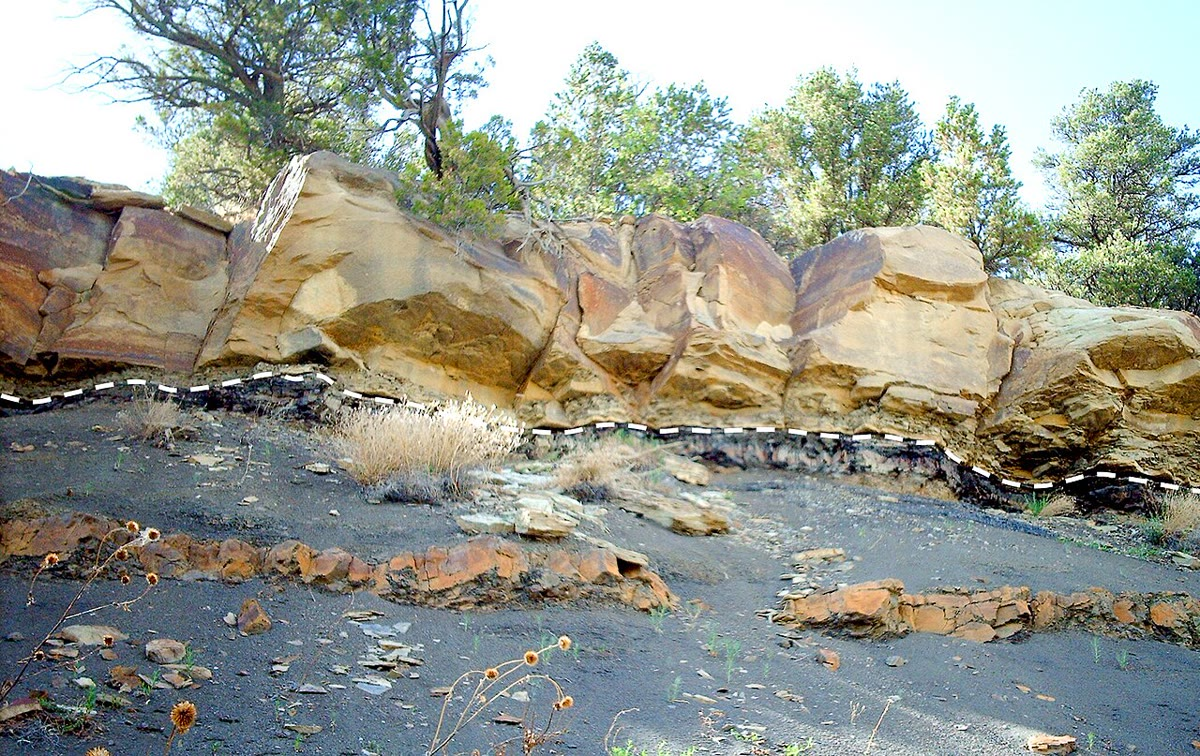
\includegraphics[width=0.78\linewidth]{images/book3/b1-kpg-boundary-trinidad.jpg}

{\small De grens tussen het Krijt en het Paleogeen, aangegeven door de gestreepte lijn, in Trinidad Lake State Park, Colorado: zandsteen erboven, donkere lagen eronder en langs de grens. (Nationalparks, CC~BY-SA~2.5, via Wikimedia Commons; de gestreepte lijn staat in het origineel.)}
\label{fig:b1:stratigraphic-scale:kpg}
\end{omfigure}
% ledger: commons:kt-tlsp

\subsection*{Het einde van het Perm}

De extinctie aan het einde van het Perm was het zwaarste verlies van mariene en landleven van het afgelopen halve miljard jaar. In Meishan in China, de sectie die het GSSP van de basis van het Trias bevat, zijn vijf asbedden gedateerd met de uranium-loodmethode op zirkoon. Zij plaatsen de extinctie tussen \qty[uncertainty-mode=separate]{251.941(37)}{\Ma} en \qty[uncertainty-mode=separate]{251.880(31)}{\Ma}: een interval van \num[uncertainty-mode=separate]{60 \pm 48} duizend jaar. Een scherpe negatieve verschuiving van \qty{3}{\permil} in de koolstofisotopen van de carbonaten gaat eraan vooraf, en de koolstofkringloop bleef ongeveer \num{500} duizend jaar onstabiel.
% ledger: burgess:end-permian, gssp:induan

De basis van het Trias zelf, \qty[uncertainty-mode=separate]{251.902(24)}{\Ma}, ligt niet bij de extinctie maar bij het eerste voorkomen van de conodont \emph{Hindeodus parvus}, een niveau dat binnen het interval van de extinctie valt dat in Meishan is gedateerd. Een extinctie is een reeks laatste voorkomens, die door de bewaring wordt vervaagd; één eerste voorkomen van een bekende soort maakt een scherpere lijn. De oorzaken van de twee extincties --- een inslag, de grote basaltprovincies --- zijn het onderwerp van Boek~4.
% ledger: gssp:induan, isg:biostratigraphy, burgess:end-permian

\section{De internationale schaal}\label{sec:b1:stratigraphic-scale:chart}

De Internationale Chronostratigrafische Schaal brengt alle eenheden, van de eonothema's tot de \omterm{def:b1:stratigraphic-scale:chronostratigraphy}{etages}, in één tabel samen: hun namen, de basis van elk in miljoenen jaren met zijn onzekerheid, een merkteken voor elke basis die door een bekrachtigd GSSP is vastgelegd, en een standaardkleur voor elke eenheid, die van de Commissie voor de Geologische Kaart van de Wereld. Het Fanerozoïcum, teruggebracht tot zijn tijdperken en perioden, wordt hieronder getekend uit de eigen waarden van de schaal.
% ledger: ics:base.Paleozoic, ics:colour.Paleozoic, gssp:count

\begin{omfigure}
\begin{tikzpicture}[font=\footnotesize]
\begin{axis}[y dir=reverse, ymin=0, ymax=538.8, xmin=0, xmax=6.2,
  width=6.6cm, height=11cm, scale only axis, clip=false,
  axis x line=none, axis y line*=left, ytick={0,100,...,500},
  ylabel={leeftijd (\unit{\Ma})}, tick label style={font=\scriptsize}]
  \pgfplotsinvokeforeach{Paleozoic,Mesozoic,Cenozoic,Cambrian,Ordovician,Silurian,Devonian,Carboniferous,Permian,Triassic,Jurassic,Cretaceous,Paleogene,Neogene,Quaternary}{
    \addplot[fill=ics#1, draw=black!70, line width=0.3pt] table[x=x, y=age] {figdata/out/bachelor-1-ics_chart-bar-#1.dat};}
  \addplot[draw=none, nodes near coords, point meta=explicit symbolic,
    every node near coord/.style={anchor=center, rotate=90, font=\scriptsize\bfseries}]
    coordinates {(0.5,395.351) [Paleozoïcum] (0.5,158.951) [Mesozoïcum] (0.5,33) [Cenozoïcum]};
  \addplot[draw=none, nodes near coords, point meta=explicit symbolic,
    every node near coord/.style={anchor=center, font=\scriptsize}]
    coordinates {(2,512.825) [Cambrium] (2,464.975) [Ordovicium] (2,431.36) [Siluur] (2,389.24) [Devoon] (2,328.88) [Carboon] (2,275.401) [Perm] (2,226.651) [Trias] (2,172.25) [Jura] (2,104.55) [Krijt] (2,44.52) [Paleogeen] (2,12.81) [Neogeen]};
  \addplot[mark=-, mark size=3pt, only marks, nodes near coords, point meta=explicit symbolic,
    every node near coord/.style={anchor=west, xshift=1pt, font=\scriptsize}]
    table[x=x, y=age, meta=lab] {figdata/out/bachelor-1-ics_chart-bases.dat};
  \addplot[only marks, mark=triangle*, mark size=3pt, mark options={rotate=90, fill=omThm, draw=omThm},
    nodes near coords, point meta=explicit symbolic,
    every node near coord/.style={anchor=west, xshift=3pt, font=\scriptsize, text=omThm}]
    coordinates {(4.75,251.902) [einde-Perm] (4.75,66) [einde-Krijt]};
  \node[anchor=south, font=\scriptsize] at (axis cs:2,0) {Kwartair};
  \node[anchor=west, font=\scriptsize] at (axis cs:3.0,-14) {0};
  \node[anchor=south, font=\scriptsize\itshape] at (axis cs:0.5,-30) {tijdperk};
  \node[anchor=south, font=\scriptsize\itshape] at (axis cs:2,-30) {periode};
  \node[anchor=south, font=\scriptsize\itshape] at (axis cs:3.5,-30) {basis (\unit{\Ma})};
\end{axis}
\end{tikzpicture}

{\small Het Fanerozoïcum op de internationale schaal: zijn drie tijdperken en twaalf perioden, op schaal, in de kleuren van de schaal, met de leeftijd van de basis van elke periode (onzekerheden weggelaten). De driehoeken markeren de twee basissen die massa-extinctiehorizonten zijn. Het Kwartair, \qty{2.58}{\Ma} lang, is de smalle strook bovenaan.}
\label{fig:b1:stratigraphic-scale:chart}
\end{omfigure}
% computed in figdata/bachelor-1/ics_chart.py; ledger: ics:base.Cambrian, ics:colour.Cambrian (every ics base and colour row of the eras and periods), burgess:end-permian, alvarez:iridium

De perioden zijn zeer ongelijk (figuur hierboven). Het Krijt duurde \qty{77.1}{\Myr}, het Neogeen \qty{20.46}{\Myr} en het Kwartair slechts \qty{2.58}{\Myr}; het gemiddelde van de twaalf is \qty{44.9}{\Myr}. De ongelijkheid is overgeërfd: de systemen werden benoemd in vroege indelingen, voordat een gesteente in jaren was gedateerd --- sommige namen geven een positie (Paleogeen, Neogeen, Kwartair), sommige een gesteente (Carboon, Krijt), sommige een volk of een plaats (Ordovicium, Siluur, Devoon, Perm) --- en de schaal behoudt de namen terwijl zij hun basis door GSSP's definieert. De leeftijden in jaren komen uit de isotopendatering van vulkanische gesteenten dicht bij de grenzen, zoals de asbedden van Meishan (\cref{ch:b1:radiometric-methods}), geïnterpoleerd zoals in \cref{prop:b1:stratigraphic-scale:interpolation}; een nieuwe versie van de schaal kan een leeftijd verschuiven terwijl het GSSP blijft waar het is.
% ledger: ics:base.Cretaceous, ics:base.Neogene, ics:base.Quaternary, isg:chronostratigraphy, burgess:end-permian

\begin{dated}{2024}
% ledger: iugs:anthropocene
Het Antropoceen, een naam die in 2001 werd voorgesteld voor een nieuw interval gekenmerkt door menselijke activiteit, werd vanaf 2009 bestudeerd door een werkgroep van de subcommissie voor kwartaire stratigrafie. Eind 2023 stelde de groep een \omterm{def:b1:stratigraphic-scale:chronostratigraphy}{serie} voor die omstreeks 1950 begint, met zijn GSSP in het sediment van Crawford Lake, Ontario. De stemming van de subcommissie, afgesloten op 4 maart 2024, verwierp het: 4 stemmen voor, 12 tegen, 3 onthoudingen, 3 leden die niet stemden. De stemgerechtigde leden van de Internationale Commissie voor Stratigrafie erkenden de stemming. Het Antropoceen is geen eenheid van de schaal; het blijft een informele term, die ruim wordt gebruikt.
\end{dated}

\section{Oefeningen}

\begin{exercise}[$\star$]\label{exo:b1:stratigraphic-scale:1}
Zeg of elke naam die van een lithostratigrafische, een biostratigrafische, een chronostratigrafische of een \omterm{def:b1:stratigraphic-scale:chronostratigraphy}{geochronologische eenheid} is, en geef zijn rang waar die er een heeft: (a)~het Jura-systeem; (b)~de Mardon \omterm{def:b1:stratigraphic-scale:lithostratigraphy}{Shale-formatie}; (c)~het Vroeg-Krijt; (d)~de \emph{Hindeodus parvus}-zone; (e)~de \omterm{def:b1:stratigraphic-scale:chronostratigraphy}{etage} Danien; (f)~het Paleoceen-tijdvak; (g)~een \omterm{def:b1:stratigraphic-scale:lithostratigraphy}{zandsteen-lid} van de Mardon Shale.
% ledger: isg:lithostratigraphy, isg:biostratigraphy, isg:chronostratigraphy
\end{exercise}

\begin{exercise}[$\star$]\label{exo:b1:stratigraphic-scale:2}
Bereken met de basis van de tijdperken in de figuur van de schaal (die van het Cambrium, het Trias en het Paleogeen) de duur van het Paleozoïcum, het Mesozoïcum en het Cenozoïcum, en het aandeel van het Fanerozoïcum dat elk vertegenwoordigt. Welk aandeel van de tijd sinds de basis van het Hadeïcum, \qty{4567}{\Ma}, vertegenwoordigt het hele Fanerozoïcum?
% ledger: ics:base.Paleozoic, ics:base.Mesozoic, ics:base.Cenozoic, ics:base.Hadean
\end{exercise}

\begin{exercise}[$\star$]\label{exo:b1:stratigraphic-scale:3}
Een klif toont, van onder af: lagen A, B, C en D, gekanteld onder \ang{40}; een dijk E die A tot D doorsnijdt; een erosieoppervlak dat de top van D en de dijk afsnijdt; horizontale lagen F en G erboven; een breuk die A tot F verplaatst, maar niet G. Zet de gebeurtenissen in volgorde, en noem het principe dat elke stap rechtvaardigt.
\end{exercise}

\begin{exercise}[$\star$]\label{exo:b1:stratigraphic-scale:4}
Twee asbedden \qty{30}{m} uit elkaar in een schalie zijn gedateerd op \qty{85.40}{\Ma} (het onderste) en \qty{84.60}{\Ma} (het bovenste). Het eerste voorkomen van een \omterm{def:b1:stratigraphic-scale:biozone}{indexfossiel} ligt \qty{12}{m} boven het onderste asbed. Bereken de accumulatiesnelheid en de leeftijd van het eerste voorkomen, uitgaande van een constante snelheid.
\end{exercise}

\begin{exercise}[$\star\star$]\label{exo:b1:stratigraphic-scale:5}
In een sectie hebben vier taxa de bereiken (hoogten in meter): A 0--34, B 12--50, C 26--62, D 41--70. (a)~Teken het bereikschema. (b)~Geef de omvang en de dikte van de zone van gelijktijdig bereik van B en C, en van de \omterm{def:b1:stratigraphic-scale:biozone}{intervalzone} tussen de eerste voorkomens van B en D. (c)~In een tweede sectie wordt B gevonden van 3 tot 15~m en C van 9 tot 22~m, en niets anders is bekend. Welke zonegrenzen van (b) zijn daar te herkennen, en welke niet? Welke horizonten kunnen met het grootste vertrouwen tussen de twee secties worden gecorreleerd?
\end{exercise}

\begin{exercise}[$\star\star$]\label{exo:b1:stratigraphic-scale:6}
Tijdens een transgressie verschoof de kustlijn landinwaarts met \qty{20}{km} per miljoen jaar. (a)~Hoeveel verschilt de leeftijd van de top van het kustzandsteen tussen twee putten \qty{60}{km} uit elkaar langs de richting van de transgressie? (b)~Een as valt één miljoen jaar nadat de kustlijn de zeewaartse put is gepasseerd, waar het slib van de zee zich opstapelt met \qty{30}{m} per miljoen jaar. Hoe ver boven de top van het zandsteen ligt het asbed dat daar wordt gevonden? (c)~Waar lag de kustlijn toen de as viel? Ligt de as boven of onder het zandsteen in de landwaartse put, en waarom kan zij daar helemaal niet worden gevonden? Verklaar met een schets.
\end{exercise}

\begin{exercise}[$\star\star$]\label{exo:b1:stratigraphic-scale:7}
(a)~Bereken de relatieve onzekerheid van de leeftijden van de basis van het Lochkovien (\qty[uncertainty-mode=separate]{419.62(136)}{\Ma}) en van het Induan (\qty[uncertainty-mode=separate]{251.902(24)}{\Ma}), in procent. Suggereer waarom zij zo sterk verschillen. (b)~Bereken uit de twee leeftijden die de extinctie aan het einde van het Perm in Meishan omsluiten, \qty[uncertainty-mode=separate]{251.941(37)}{\Ma} en \qty[uncertainty-mode=separate]{251.880(31)}{\Ma}, opnieuw de duur van de extinctie en haar onzekerheid, uitgaande van twee onafhankelijke fouten. Vergelijk met de gepubliceerde \num[uncertainty-mode=separate]{60 \pm 48} duizend jaar.
% ledger: ics:base.Devonian, gssp:induan, burgess:end-permian
\end{exercise}

\begin{exercise}[$\star\star$]\label{exo:b1:stratigraphic-scale:8}
Neem de asteroïde van 1980 als een bol van \qty{10}{km} breed, met een dichtheid van \qty{3000}{kg.m^{-3}} (een aangenomen waarde), die 60 keer zijn massa aan stof opwerpt. (a)~Bereken de massa van de asteroïde en van het stof. (b)~Verspreid het stof gelijkmatig over de aarde (diameter \qty{12756}{km}): welke massa valt op elke vierkante meter? (c)~Afgezet met een dichtheid van \qty{2500}{kg.m^{-3}}, hoe dik is de laag? (d)~Herhaal (c) voor diameters van \qty{6}{km} en \qty{14}{km}, het bereik van de schatting. Vergelijk met de dikte van de grensklei bij het GSSP van het Danien.
% ledger: alvarez:iridium, planet:Earth.diameter, gssp:danian
\end{exercise}

\begin{exercise}[$\star\star$]\label{exo:b1:stratigraphic-scale:9}
(a)~In een condenserend profiel waar het sediment \qty{2}{m} per miljoen jaar ophoopte, hoe dik is het interval van \num{60} duizend jaar van de extinctie aan het einde van het Perm? Hoe dik zou het zijn voor de kortste en de langste duur die door de onzekerheid is toegestaan? (b)~In een diepzeeprofiel dat met \qty{10}{m} per miljoen jaar ophoopt, hoe dik is het interval van \num{32000} jaar waarbinnen de inslag en de K--Pg-grens gelijktijdig zijn? (c)~Wat zeggen deze getallen over het bemonsteren van een sectie om een extinctie te bestuderen?
% ledger: burgess:end-permian, renne:kpg
\end{exercise}

\begin{exercise}[$\star\star\star$]\label{exo:b1:stratigraphic-scale:10}
Een kustvlakte helt $1$ op $2000$ en het \omterm{def:b1:diagenesis-basins:eustasy}{relatief zeeniveau} stijgt met \qty{10}{m} per miljoen jaar. (a)~Hoe snel verschuift de kustlijn met \cref{prop:b1:stratigraphic-scale:transgression} landinwaarts, en met hoeveel verschilt de leeftijd van de top van het kustzandsteen tussen twee putten \qty{30}{km} uit elkaar? (b)~Er wordt nu sediment naar de kust aangevoerd, dat de kustvlakte bij de kustlijn met $a$ meter per miljoen jaar omhoog bouwt. Toon aan dat de kustlijn met $(R - a)/s$ landinwaarts beweegt zolang $a < R$. Wat gebeurt er wanneer $a > R$? (c)~Verklaar waarom een zandsteentop waarvan de leeftijd met een miljoen jaar verandert, in één klif er precies uit kan zien als een oppervlak van gelijke leeftijd.
\end{exercise}

\begin{exercise}[$\star\star\star$]\label{exo:b1:stratigraphic-scale:11}
Twee asbedden liggen op \qty{10}{m} en \qty{50}{m} in een sectie en zijn gedateerd op \qty[uncertainty-mode=separate]{100.50(5)}{\Ma} en \qty[uncertainty-mode=separate]{99.70(3)}{\Ma}. (a)~Interpoleer de leeftijd van een niveau op \qty{25}{m} en zijn onzekerheid met \cref{prop:b1:stratigraphic-scale:interpolation}. (b)~Waar tussen de twee assen is de onzekerheid het kleinst? Vind de waarde van $f$ die $\sigma_t$ minimaliseert, en het minimum. (c)~Toon aan dat $\sigma_t$ tussen de twee lagen nooit de grootste van $\sigma_1$ en $\sigma_2$ overschrijdt.
\end{exercise}

\begin{exercise}[$\star\star\star$]\label{exo:b1:stratigraphic-scale:12}
Een put doorkruist een uniforme schalie. Een as gedateerd op \qty{30.0}{\Ma} ligt op \qty{1000}{m} diepte en een as gedateerd op \qty{29.0}{\Ma} op \qty{200}{m}; een grens van een \omterm{def:b1:stratigraphic-scale:chronostratigraphy}{etage} ligt op \qty{600}{m}. (a)~Interpoleer haar leeftijd uit de dieptes. (b)~De korrels, niet de poriën, kwamen met een constante snelheid aan. Gebruik de schalie van \cref{tab:b1:diagenesis-basins:athy} en \cref{prop:b1:diagenesis-basins:solid}, bereken de vaste dikte tussen elke as en de grens, en interpoleer de leeftijd opnieuw in verhouding daarmee. (c)~Met hoeveel duizend jaar verschillen de twee schattingen, en welke is de betere?
% ledger: pybacktrack:compaction
\end{exercise}

\section{Probleem: drie secties over een bekken correleren}

\begin{problem}[{Weekendprobleem --- hoe fossielen, asbedden en een diachrone
zandsteen samen een etagegrens dateren}]
\label{pb:b1:stratigraphic-scale:1}
% values: calc/ch24.py; the basin, its sections, its taxa (Vardenoceras and Ostreola) and its ash ages are invented
Drie secties worden langs een lijn over een verzonnen bekken gelogd: A in het westen, B \qty{25}{km} oostelijk van A, en C \qty{20}{km} oostelijk van B. In elk ligt de Kell Sandstone onder de Mardon Shale. Hoogten zijn in meter boven de basis van elke sectie:
\begin{center}
\small
\begin{tabular}{lccc}
\hline
 & A & B & C \\
\hline
totale gelogde dikte                         & 80.0 & 66.0 & 32.0 \\
top van de Kell Sandstone                    & 45.0 & 20.0 & 6.0 \\
asbed 1 (gedateerd op \qty[uncertainty-mode=separate]{152.40(4)}{\Ma})  & 5.0  & 8.0  & 3.0 \\
asbed 2 (gedateerd op \qty[uncertainty-mode=separate]{151.20(4)}{\Ma})  & 71.0 & 56.0 & 27.0 \\
eerste voorkomen van \emph{Vardenoceras medium} & 36.6 & 31.2 & 14.8 \\
eerste voorkomen van \emph{Vardenoceras ultimum} & 65.8 & 52.0 & 24.8 \\
laatste voorkomen van \emph{Vardenoceras primum}   & 49.0 & 40.0 & 19.0 \\
\hline
\end{tabular}
\end{center}
\emph{V.~primum} wordt vanaf de basis van elke sectie gevonden. De tweekleppige \emph{Ostreola} wordt alleen in de Kell Sandstone gevonden, in alle drie secties. Drie \omterm{def:b1:stratigraphic-scale:biozone}{intervalzones} worden gedefinieerd: zone~1 tot het eerste voorkomen van \emph{V.~medium}, zone~2 tot dat van \emph{V.~ultimum}, zone~3 erboven. Een etagegrens wordt, bij haar GSSP elders, gedefinieerd door het eerste voorkomen van \emph{V.~medium}.

\medskip
\noindent\textbf{Deel I --- Biozones.}
\begin{enumerate}
  \item Teken de drie secties naast elkaar op een gemeenschappelijke verticale schaal, met de Kell Sandstone, de asbedden en de zonegrenzen.
  \item Geef de dikte van zone~2 in elke sectie, en de dikte van het deel van zone~3 dat is gelogd.
  \item Waarom kan de basis van zone~1 in geen van de drie secties worden geplaatst?
  \item Waarom is \emph{Ostreola} een slecht \omterm{def:b1:stratigraphic-scale:biozone}{indexfossiel}, hoe algemeen het ook is?
  \item In welke zone valt het laatste voorkomen van \emph{V.~primum} in elke sectie? Zou het een vierde zonegrens kunnen zijn?
  \item Correleer de secties via de eerste voorkomens van \emph{V.~medium} en \emph{V.~ultimum}. Wat suggereert de verhouding van de diktes van zone~2?
\end{enumerate}

\noindent\textbf{Deel II --- De Kell Sandstone.}
\begin{enumerate}[resume]
  \item In welke zone ligt de top van de Kell Sandstone in elke sectie?
  \item Is de top van de Kell Sandstone een oppervlak van gelijke leeftijd? In welke richting verschoof de kustlijn, en wat voor gebeurtenis is dit?
  \item Asbed~1 ligt in alle drie secties in de Kell Sandstone, asbed~2 in de Mardon Shale. Waarom zijn de asbedden betere tijdlijnen dan de grens van de \omterm{def:b1:stratigraphic-scale:lithostratigraphy}{formatie}?
  \item Welke van de principes van \cref{def:b1:stratigraphic-scale:principles} rechtvaardigen het volgen van één asbed van A tot C?
\end{enumerate}

\noindent\textbf{Deel III --- Snelheden.}
\begin{enumerate}[resume]
  \item Bereken de accumulatiesnelheid tussen de twee asbedden in elke sectie, in meter per miljoen jaar.
  \item Suggereer waarom de snelheid van A naar C daalt.
  \item Hoeveel jaar vertegenwoordigt een monster van \qty{10}{cm} dik in elke sectie? Welke sectie geeft de fijnste resolutie in de tijd?
  \item Bereken, uitgaande van constante snelheden, de leeftijd van de top van de Kell Sandstone in elke sectie.
  \item Bereken de snelheid van de kustlijn tussen C en B en tussen B en A, in kilometer per miljoen jaar. Versnelde de transgressie of vertraagde zij?
  \item Bereken de leeftijd van het eerste voorkomen van \emph{V.~ultimum} in elke sectie.
  \item Komen de drie leeftijden van vraag~16 overeen binnen de onzekerheid van de asdateringen? Wat zegt dit over het eerste voorkomen?
\end{enumerate}

\noindent\textbf{Deel IV --- De leeftijd van de grens.}
\begin{enumerate}[resume]
  \item Interpoleer, in elke sectie, de leeftijd van het eerste voorkomen van \emph{V.~medium}.
  \item Bereken de onzekerheid van elke leeftijd uit de onzekerheden van de asdateringen met \cref{prop:b1:stratigraphic-scale:interpolation}.
  \item Bereken het gemiddelde van de drie leeftijden en hun spreiding. Is de spreiding groter of kleiner dan de onzekerheid van vraag~19?
  \item In sectie~A ligt het eerste voorkomen van \emph{V.~medium} in de Kell Sandstone, in B en C in de Mardon Shale. Hoe kan een verandering van lithologie tussen de asbedden de interpolatie in A vertekenen?
  \item Welke van de drie secties zou het beste \omterm{def:b1:stratigraphic-scale:gssp}{grensstratotype} zijn, en waarom? Welke zou de slechtste zijn?
  \item Hoe lang duurde zone~2?
  \item Wat is de geïnterpoleerde leeftijd van de grens?
\end{enumerate}
\end{problem}
